\documentclass[12pt,a4paper]{article}
\usepackage[utf8]{inputenc}
\usepackage[brazilian]{babel}
\usepackage{amsmath}
\usepackage{amsfonts}
\usepackage{amssymb}
\usepackage[T1]{fontenc}
\usepackage{graphicx}
\usepackage{physics}
\usepackage{float}

\usepackage{siunitx}
\newcounter{prob}
\newcounter{subprob}
\renewcommand{\thesubprob}{\alph{subprob}}

\newcommand{\problem}[1]{\setcounter{subprob}{0} \stepcounter{prob} \par \medskip \noindent \textbf{#1 \ .}}

\newcommand{\answer}{\par \medskip \noindent \textit{\textbf{prova} \ }}

\newcommand{\finalanswer}[1]{
	\begin{center} 
    	{\renewcommand{\arraystretch}{1.5}
		\renewcommand{\tabcolsep}{0.2cm} 
    	\begin{tabular}{|c|} 
    		\hline 
        	$ \displaystyle #1 $  \\ 
        	\hline 
    	\end{tabular}} 
   	\end{center}}

\newcommand{\subproblem}[1]{ \par \smallskip \noindent \quad \textit{(#1)  \ }}

\newcommand{\subanswer}{\par \smallskip \noindent \quad \textit{ \ }}

\newcommand{\option}{\item[$\square$]}
\newcommand{\thisone}{\item[$\blacksquare$]}

\newenvironment{subitemize}{\begin{itemize}}{\end{itemize}}


\author{Leonardo Mendes de Moraes }
\title{Lista 4 - MAC5711}
\date{}
\begin{document}

%%--CABEÇALHO--%%
	\begin{center}
    {\huge Lista 4 \par} {\LARGE Análise de Algoritmos \par} {\Large MAC5711
    \par}
	\end{center}

\problem{1} Suponha que $A[1...m]$ é um heap e que $1 < i \leq j \leq m$.
    Prove ou forneça um contra-exemplo para as seguintes afirmações:
    \subproblem{a} Se $A[i] < A[j]$ e os valores de $A[i]$ e $A[j]$ forem
    trocados, $A[1..m]$ continuará sendo um heap? \\
    A propriedade do heap é:
    \begin{equation}
            A[i/2] \geq A[i]
        \notag
    \end{equation}
    Portanto, $A[1..m]$ só permanecerá sendo um heap se a troca de $A[i]$ com
    $A[j]$ não interferir com a propriedade acima. Ou seja, $A[i]$ tem que ser
    maior que o valor de $A[2i]$ e $A[2i + 1]$, e $A[j]$ maior que $A[2j]$ e
    $A[2j +1]$. O heap definido abaixo, por exemplo:
    \begin{figure}[H]
        \centering

        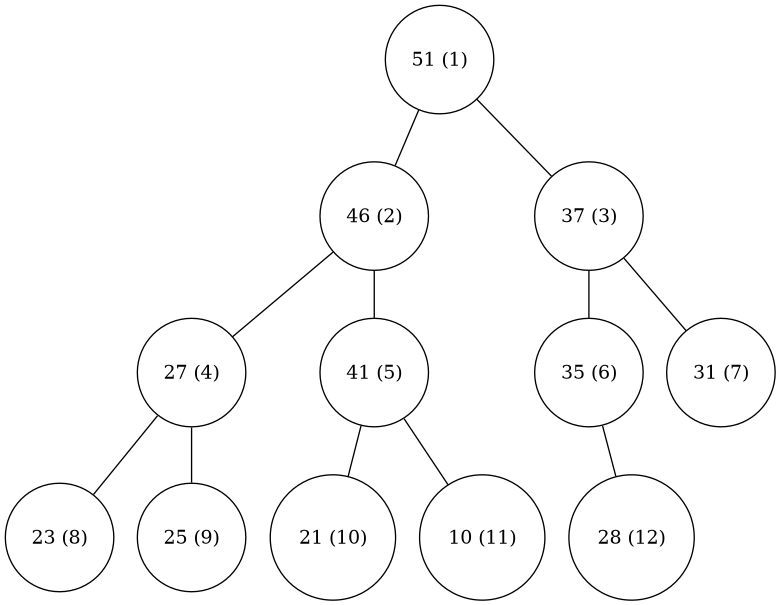
\includegraphics[scale=0.4]{heap1.png}
    \end{figure}

    Se definirmos $i$ e $j$ como $3$ e $5$, respectivamente, e fizermos a troca, temos:

    \begin{figure}[H]
        \centering

        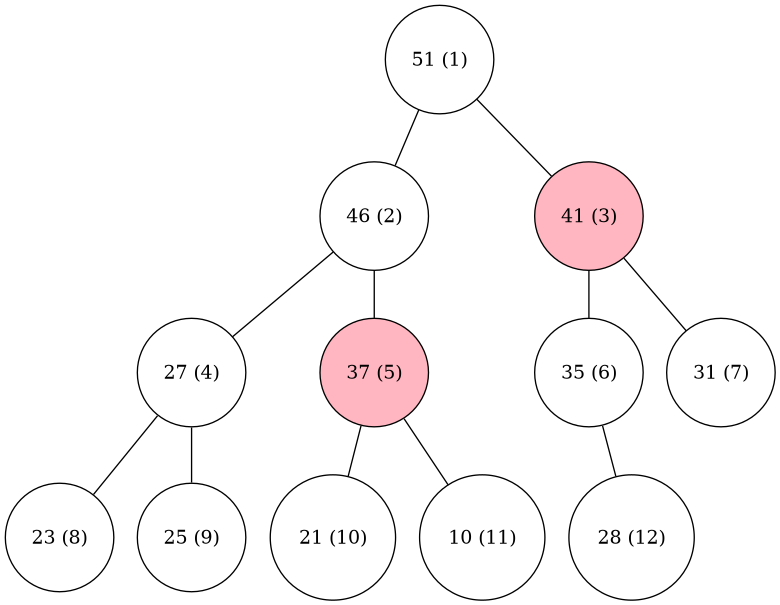
\includegraphics[scale=0.4]{heap2.png}
    \end{figure}

    Portanto, nesse caso ambos os nós mantiveram suas propriedades, logo,
    $A[1..m]$ continua sendo um heap.

    Se pegarmos o heap original e definirmos $i$ e $j$ como  $4$ e $6$, temos:

    \begin{figure}[H]
        \centering

        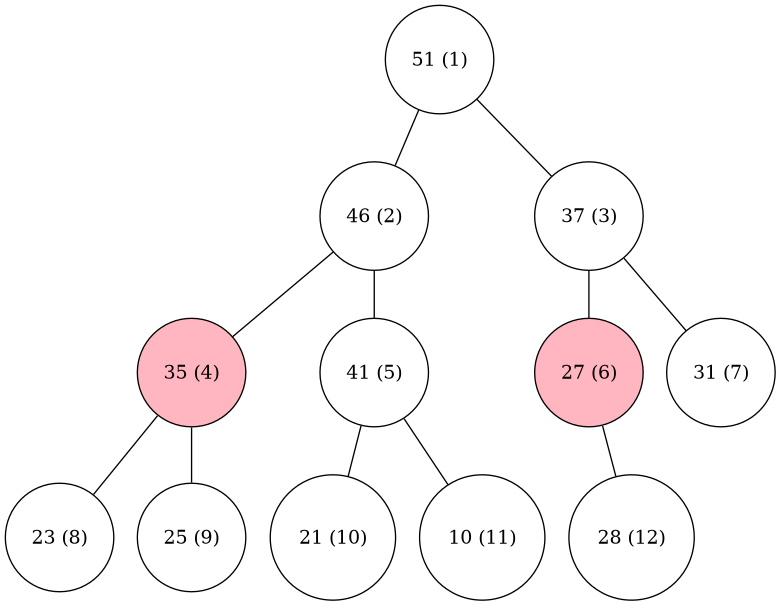
\includegraphics[scale=0.4]{heap3.png}
    \end{figure}

    Aqui, pode-se ver que a propriedade do heap não se manteve pois o nó $6$ é
    menor que o nó $12$.

    Portanto, pode-se concluir que depende se a troca mantém a propriedade no
    caso de $A[j]$.

    \subproblem{b} Se $A[i] > A[j]$ e os valores de $A[i]$ e
    $A[j]$ forem trocados, $A[1 . . m]$ continuará sendo um heap?

    Assim como acima, $A[1..m]$ se manterá um heap se na troca, $A[i]$ manter a
    propriedade, ou seja, se o valor inicial de $A[j]$ é maior que $A[2i]$ e
    $A[2i + 1]$.

    \problem{9}

\end{document}